\documentclass{beamer}

\usepackage[utf8]{inputenc}
\usepackage[T1]{fontenc}
\usepackage[english]{babel}
\usepackage{lmodern}
\usepackage{color}
\usepackage{fix-cm}
\usepackage{textpos}
\usepackage{eurosym}
\usepackage{multirow}
\usepackage{perpage}

% Redéfinis les marges des tableaux
\let\oldtabular=\tabular
\def\tabular{\small\oldtabular}
\renewcommand{\arraystretch}{1.5}

\usetheme{Warsaw}
\usecolortheme{orchid}

% Permet de réinitialiser les footnote à chaque frame. Nécéssite 2 compilations.
\MakePerPage{footnote}

\setlength{\TPHorizModule}{0.01\textwidth}
\setlength{\TPVertModule}{0.01\textheight}

\setbeamertemplate{navigation symbols}{}

\title[Elon Musk's strategies to not die on earth]{
    How Elon Musk, with his strategies, wants to bring our civilization to the
    next level?
}
\author[HOUDAYER \and KIM \and RUHIER]{
	Benoit HOUDAYER\\
    \and
    Pauline KIM\\
    \and
	Anthony RUHIER
}
\institute[LE84 - UTBM]{
    Business english (LE84) - Université Technologique de Belfort Montbéliard}
\date{January 2016}

\begin{document}

% Permet de masquer le comptage de slides
\bgroup
\makeatletter
\setbeamertemplate{headline}{}
\setbeamertemplate{footline}
{
  \leavevmode%
  \hbox{%
  \begin{beamercolorbox}[wd=.5\paperwidth,ht=2.25ex,dp=1ex,center]{title in head/foot}%
    \usebeamerfont{title in head/foot}\insertshorttitle
  \end{beamercolorbox}%
  \begin{beamercolorbox}[wd=.5\paperwidth,ht=2.25ex,dp=1ex,center]{date in head/foot}%
    \usebeamerfont{date in head/foot}\insertshortdate{}
%    \insertframenumber{} / \inserttotalframenumber\hspace*{2ex}
  \end{beamercolorbox}}%
}
\makeatother

\begin{frame}[noframenumbering]
 	\frametitle{}
	\titlepage
\end{frame}
\egroup

\begin{frame}[noframenumbering,plain]
    I want Iron Man to punch the Hulk here!
	% \begin{textblock}{0}(5,-5)
    %     \center{\includegraphics[width=.7\paperwidth]{images/logo-fsf.eps}}
	% \end{textblock}
\end{frame}

\logo{
\includegraphics[height=1cm]{images/logo-utbm.eps}\hspace*{2em}}


% Ajout du compteur de slides
\expandafter\def\expandafter\insertshorttitle\expandafter{%
      \insertshorttitle\hfill%
      \insertframenumber\,/\,\inserttotalframenumber}

\begin{frame}
	\begin{small}
	\frametitle{Sommaire}
	\tableofcontents
	\end{small}
\end{frame}

\AtBeginSection[]
{
	\begin{small}
	\begin{frame}
		\frametitle{Sommaire}
		\tableofcontents[currentsection]
	\end{frame}
	\end{small}
}


%%%% Includes des sections :
%%%%%%%%%%%%%%%%%%%%%%%%%%%%%%
%
    \section{Global vision}

\subsection{Character sheets}
\begin{frame}
\frametitle{Character sheets}
\begin{itemize}
    \itemsep2em
    \begin{columns}
        \begin{column}{40mm}
        \item South African from a modest family
        \item PhD in applied physics at Stanford
        \item US \${}12.4 billion in 2016
        \end{column}
        \begin{column}{35mm}
        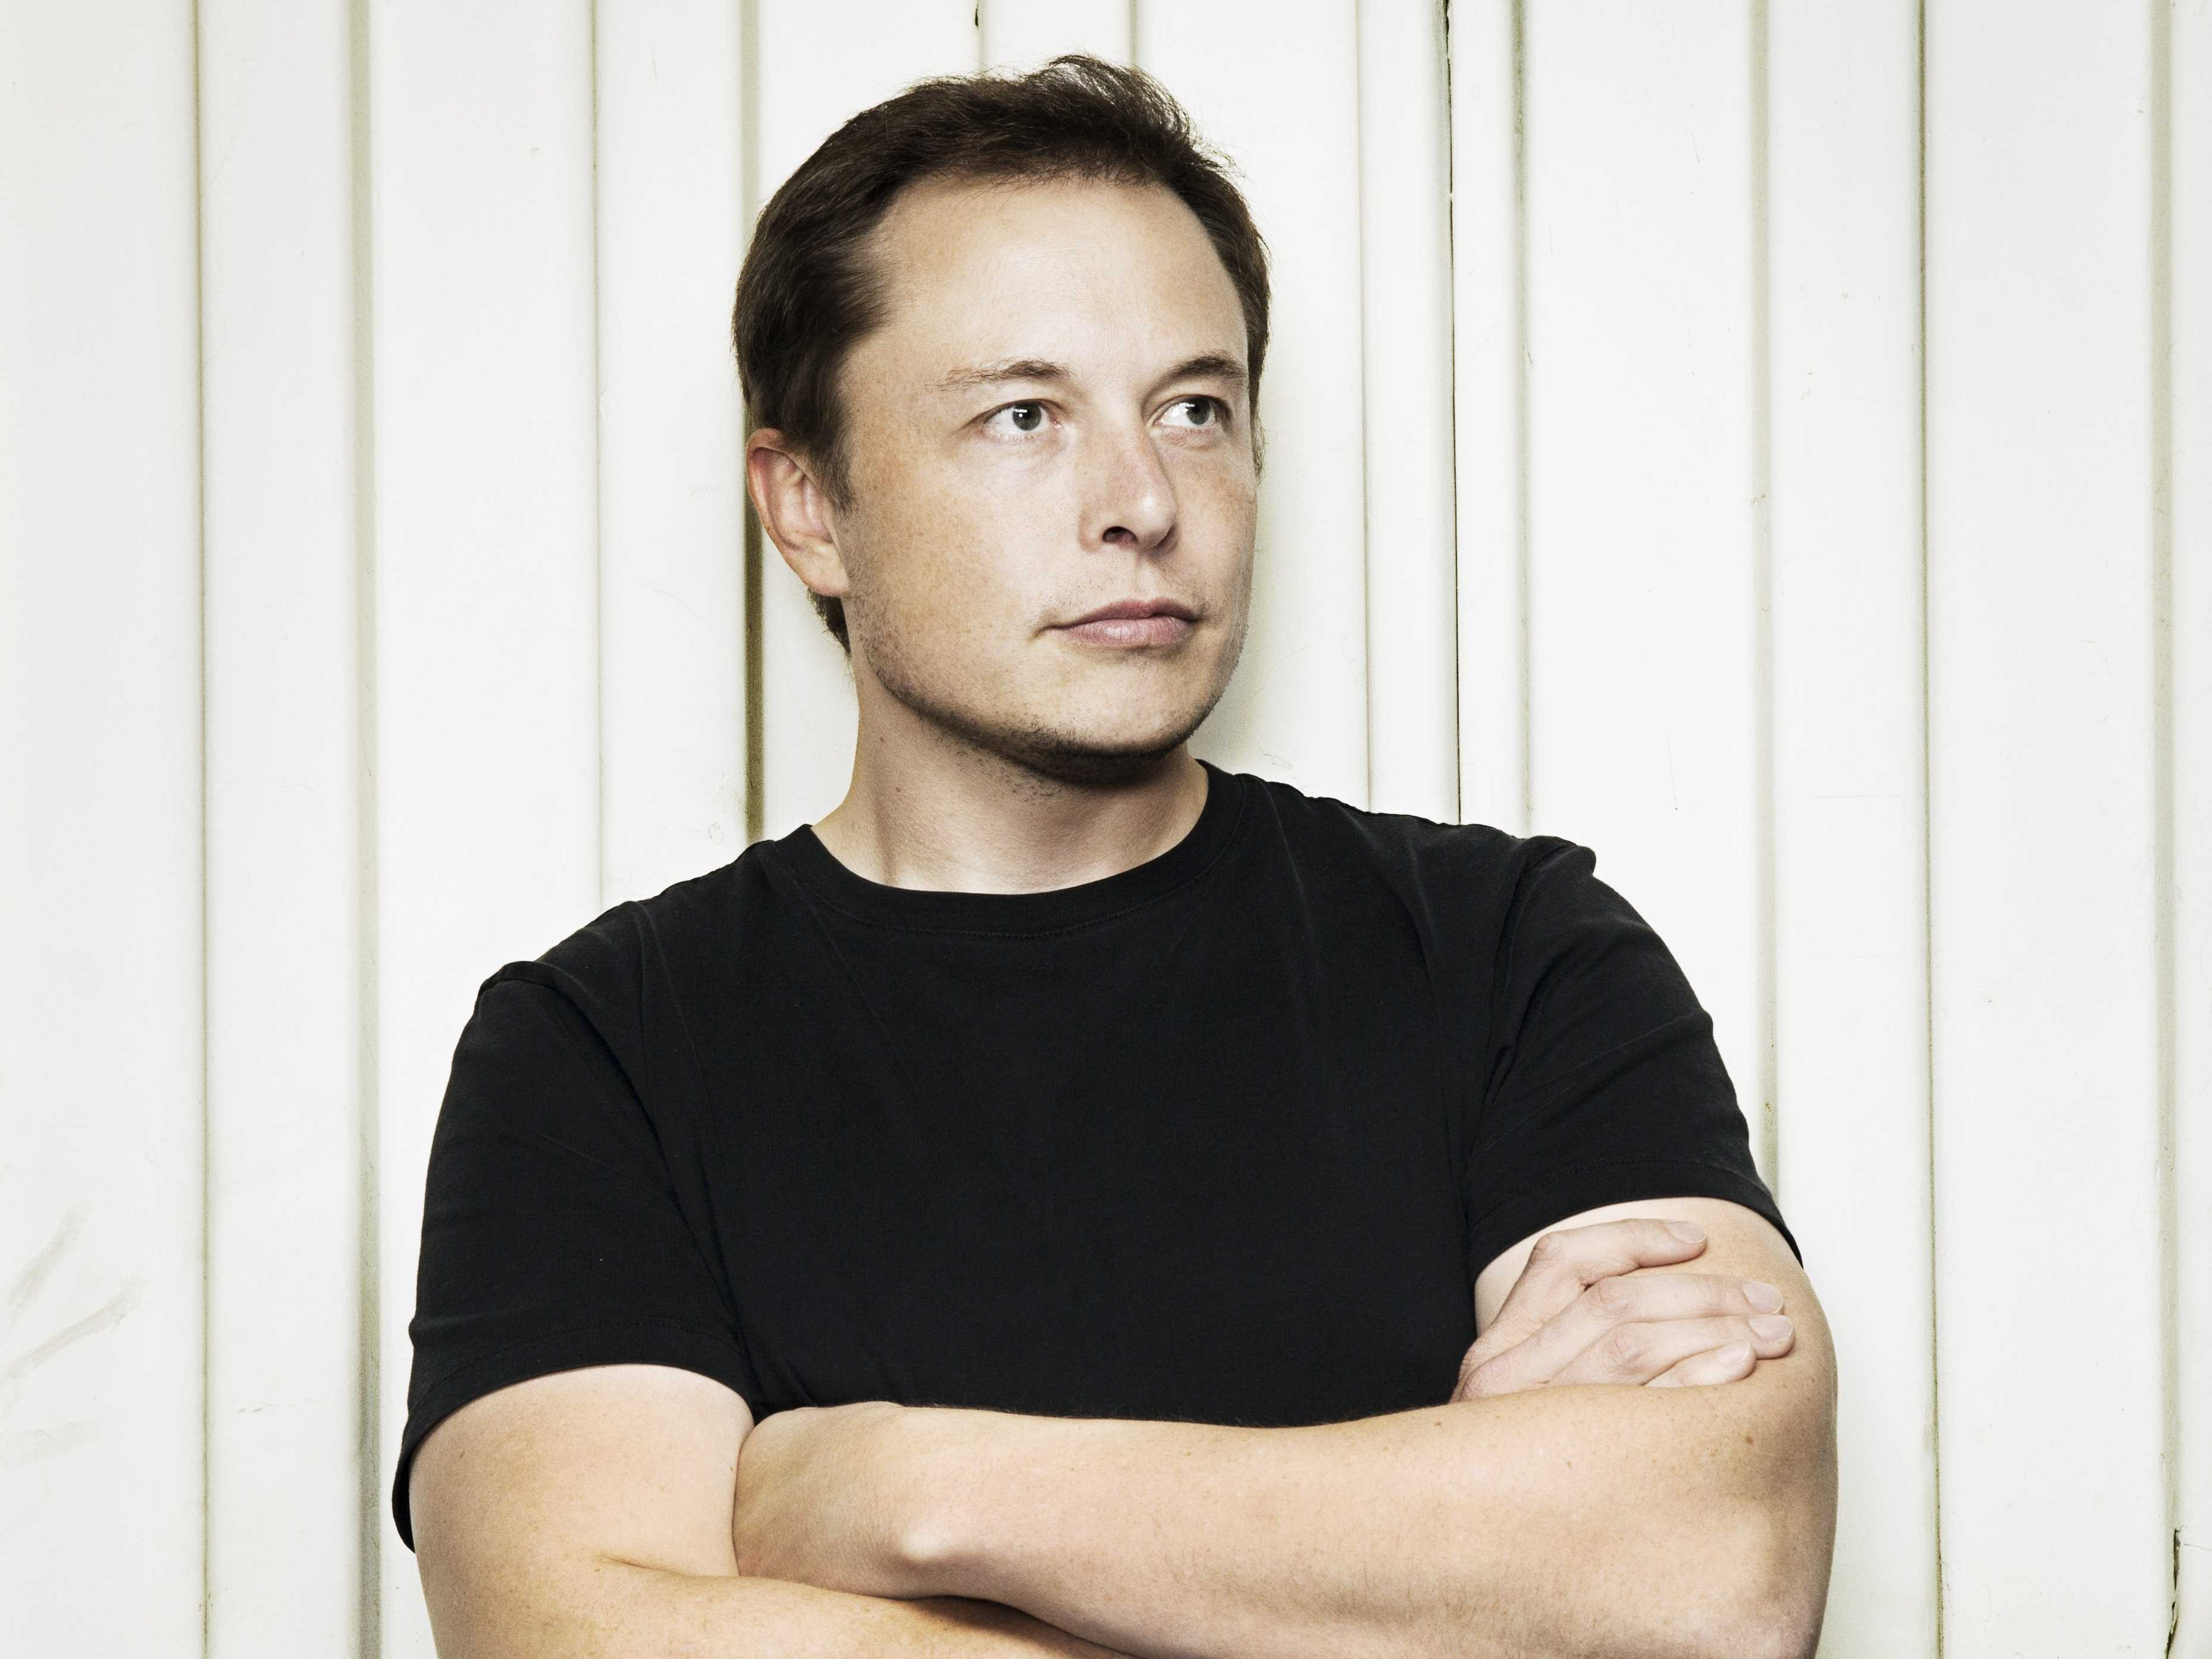
\includegraphics[width=45mm]{images/musk.jpg}
        \end{column}
    \end{columns}
    \item Does not want to die on Earth
\end{itemize}
\end{frame}


\subsection{Carrier}
\begin{frame}
\frametitle{Carrier}
\begin{itemize}
    \itemsep1em
    \item Zip2, co-founded in 1995
    \item Paypal, co-founded in 1999
    \item CEO and CTO of SpaceX, founded in 2001
    \item CEO and CTO of Tesla Motors, founded in 2003
    \item Chairman of SolarCity, founded in 2006
    \item Hyperloop, concept created in 2014
    \item Co-chairman of OpenAI, co-founded in 2015
\end{itemize}
\end{frame}


\subsection{Long term goals}
\begin{frame}
\frametitle{Long term goals}
\begin{itemize}
    \itemsep1.5em
    \item Breaking the legacies of transportation technologies
    \item Traveling on Mars
    \item Stop using fossil fuels as our main power source
    \item Avoid the humanity to die before the next 2 centuries
\end{itemize}
\end{frame}


\begin{frame}
\frametitle{Transportation technologies}
\begin{itemize}
    \itemsep1em
    \item Electric cars with Tesla Motors
    \item Add a transportation system between trains and planes, with the
        Hyperloop
    \item Reusable rockets, able to land, because:
        \begin{quote}
            ``Obviously it'd be kind of weird if the aliens landed in the ocean
            with parachutes, we'd be like okay, nothing to fear.'' Elon Musk to
            a journalist.
        \end{quote}
\end{itemize}
\end{frame}

    \section{Tesla Motors}

\subsection{A little bit of history}
\begin{frame}
\frametitle{A little bit of history}
\begin{itemize}
    \itemsep1em
    \item Cars were powered by electricity in 1903
    \item Ford needed to reduce the production costs of thermal engines
    \item Developing a new way to produce faster % mass production
    \item Seems to have worked since 1908 and the Ford T
    \item Product advertisement was not needed between 1917 and 1923
\end{itemize}
\end{frame}

\subsection{The weird kid in the playground}
\begin{frame}
\frametitle{Everyone wants an electric car}
\begin{itemize}
    \itemsep1.5em
    \item Smooth feeling on the road
    \item Decrease the dependency to oil
    \item Reduces the pollution released compares to classic cars
    \item Everybody seems to agree it is the future car
\end{itemize}
\end{frame}

\begin{frame}
\frametitle{But…}
\begin{itemize}
    \itemsep1.5em
    \item What about the autonomy?
    \item The drive might be slow… no?
    \item Reducing the pollution… really? % preconceived ideas
    \item OK but… it has to be today? Not… like… tomorrow?
\end{itemize}
\end{frame}

\begin{frame}
\frametitle{No one wants electric cars to be on the market}
\begin{itemize}
    \itemsep1.5em
    \item Selling classic cars would be difficult % 10 parts compared to 200
    \item Requires investments
    \item Lobbying by the oil industry
    \item Governments are not pushing it enough
\end{itemize}
\end{frame}


\subsection{A plan in 3 big steps}

\begin{frame}
\frametitle{Electric cars can be cool}
\begin{itemize}
    \itemsep1.5em
    \item Supercar: roadster
    \item Powerful: 0–60 mph of 3.70 seconds and a quarter-mile test at 12.6 sec @ 102.6 mph (165.1 km/h)
    \item US\$128,500
    \item No compromise
    \item Regular cool upgrades
    % At this step, Musk has to reinvest a big part of his money or tesla would
    % die
\end{itemize}
\end{frame}


\begin{frame}
\frametitle{Electric cars can be classy}
\begin{itemize}
    \itemsep1.5em
    \item Model S and then Model X
    \item More ``affordable'': US\$80,000
    \item Range: 320 miles (520km)
    \item Autopilot and cool features
    \item Really good reviews
\end{itemize}
\end{frame}


\begin{frame}
\frametitle{Not only super rich peoples can buy a good electric car}
\begin{itemize}
    \itemsep1.5em
    \item Model X
    \item Should be on the market in 2017
    \item Should cost around US\$40,000
    \item Not the car for everyone, but a big step
\end{itemize}
\end{frame}

\section{SpaceX}

{
\logo{}
\subsection{Why SpaceX exists}

\begin{frame}
\frametitle{Why SpaceX Exists}

    \begin{columns}
        \begin{column}{45mm}
        The ultimate goal : \\Colonise Mars (no less)
        \end{column}
        \begin{column}{65mm}
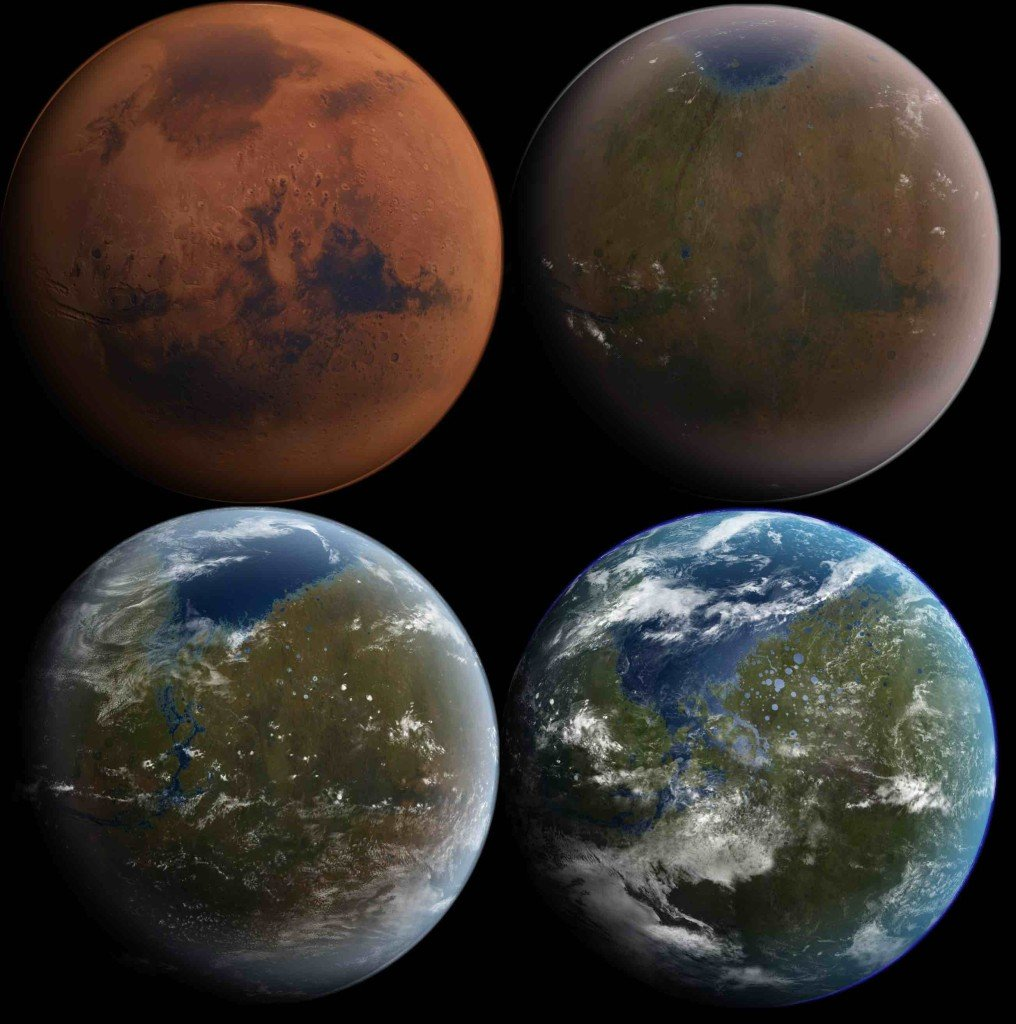
\includegraphics[width=65mm]{images/mars_transition}
        \end{column}
    \end{columns}
\end{frame}
}


\subsection{The Problem}

\begin{frame}
    \frametitle{The Problem}
    \begin{itemize}
        \item 1M people needed for autonomous colony \pause
        \item current Mars shuttle holds 6 \pause
        \item costs 50 M\$ per passenger
    \end{itemize}
\end{frame}

\begin{frame}
    \frametitle{The Solution}
    \begin{enumerate}
        \item Learn rocket science
        \pause
        \item Make cost-effective rockets
        \pause
        \item Put payloads in orbit $\rightarrow$ experience and profit
        \pause
        \item Bring Mars flight ticket to 500 000 \$
        \pause
        \item Send people by batches of 100
    \end{enumerate}
\end{frame}

\subsection{SpaceX History}

\begin{frame}
    \frametitle{SpaceX History}

    \begin{itemize}
        \item 2006 - first launch  $\rightarrow$ failure
        \item 2007 - second launch $\rightarrow$ failure
        \item 2008 - third launch  $\rightarrow$ failure

    \end{itemize}
    \vspace{1em}
    \pause

    september 2008\\
    last try before running out of funds\\
    \begin{itemize}
        \item success $\rightarrow$ 1.6 B\$ contract with NASA
    \end{itemize}
\end{frame}

\subsection{SpaceX's Technology}

{
    \logo{}

\begin{frame}
    \frametitle{SpaceX's Current Technology}
    \begin{columns}
        \begin{column}{60mm}
            The merlin engine :\\
            \vspace{1em}
            \begin{itemize}
                \item mass : 440 kg
                \item thrust : 716 kN ($\simeq$73 Tons)
                \item thrust-to-weight ratio : 165.9
            \end{itemize}
        \end{column}
        \begin{column}{45mm}
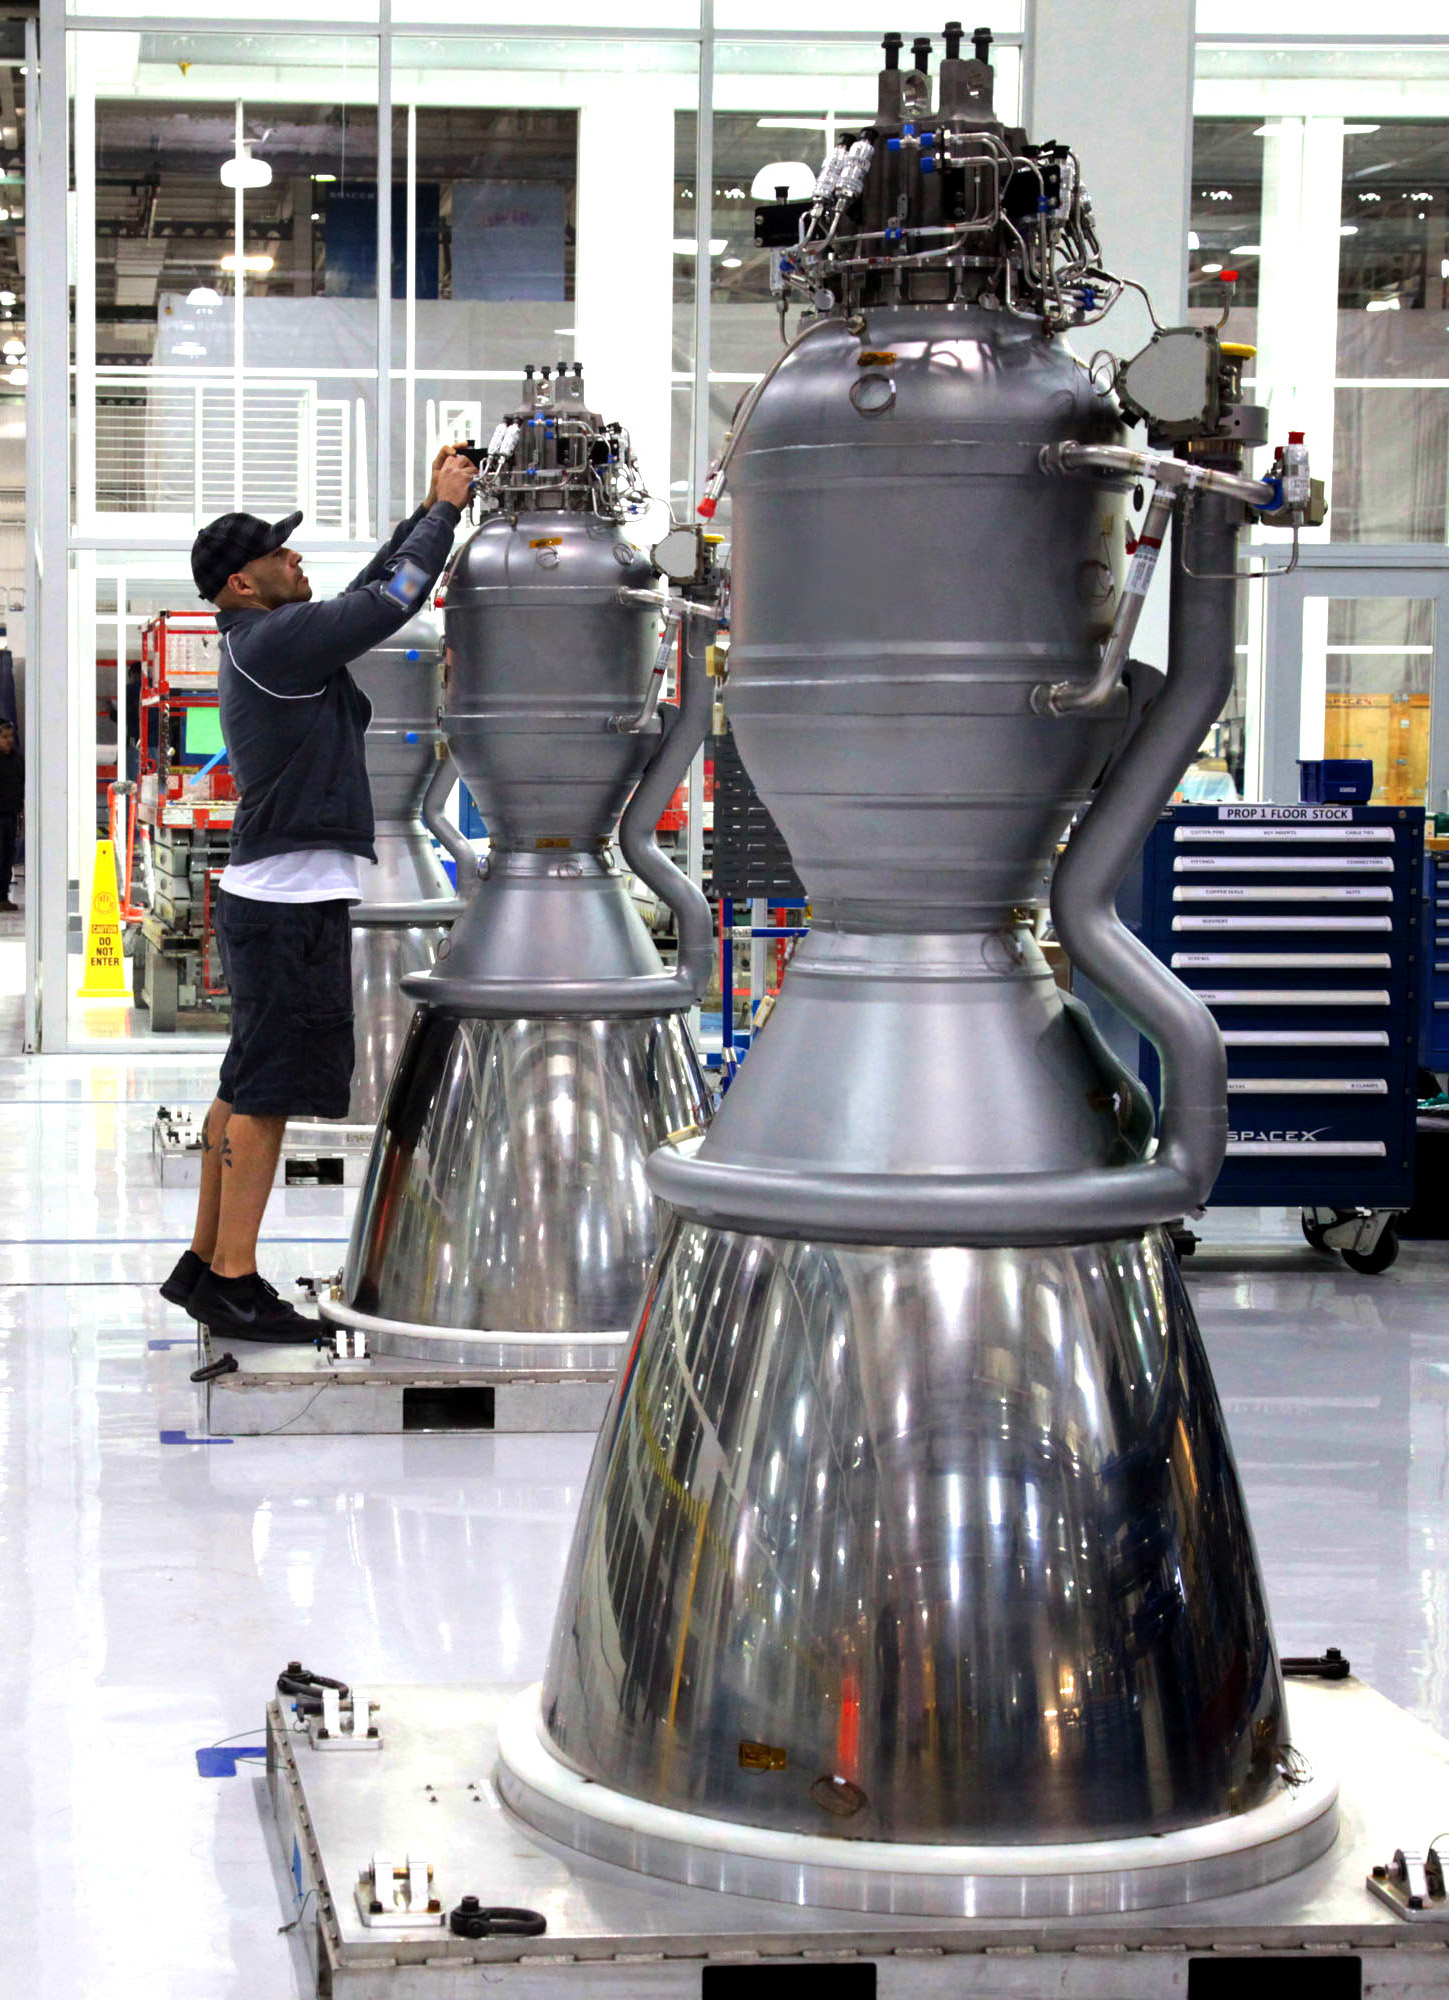
\includegraphics[width=48mm]{images/shiny_merlin}
        \end{column}
    \end{columns}
\end{frame}

\begin{frame}
    \frametitle{SpaceX's Current technology}
    \begin{columns}
        \begin{column}{60mm}
            The falcon 9 :\\
            \vspace{1em}
            \begin{itemize}
                \item 68m high
                \item 13 tons of payload to LEO
                \item active since 2010
                \item uses 9 Merlins \\(hence the name)
            \end{itemize}
        \end{column}
        \begin{column}{50mm}
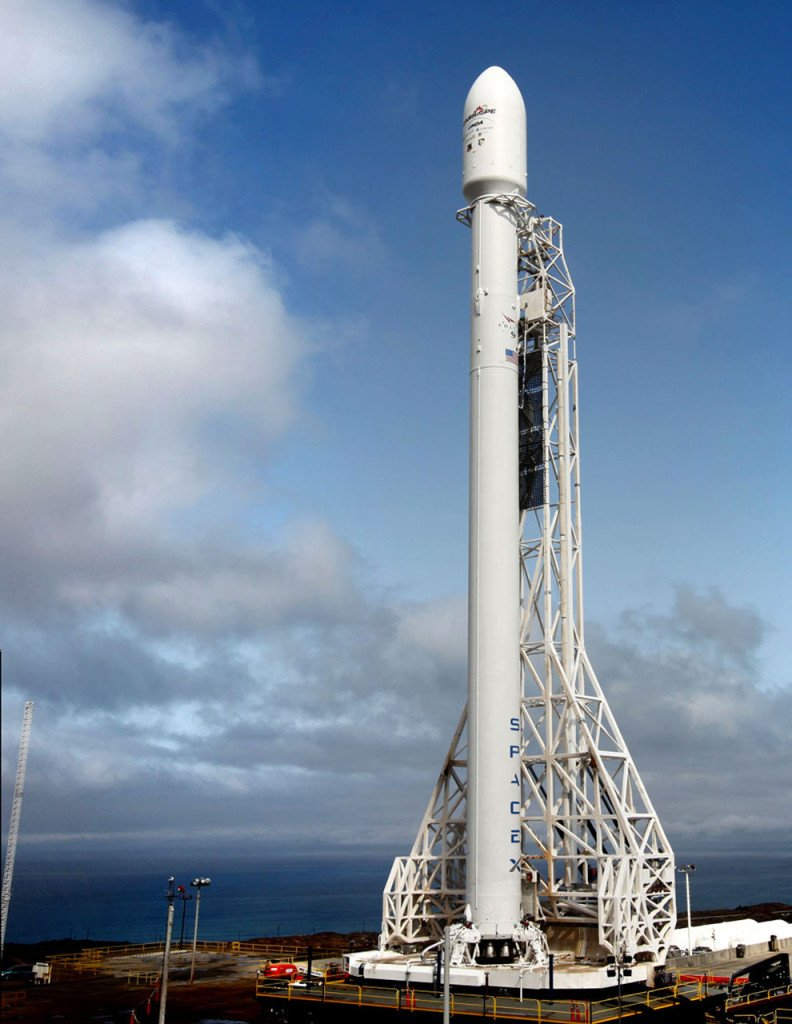
\includegraphics[height=66mm]{images/falcon9}
        \end{column}
    \end{columns}
\end{frame}

\begin{frame}
    \frametitle{SpaceX's Current technology}
    \begin{columns}
        \begin{column}{50mm}
            Dragon :\\
            \vspace{1em}
            \begin{itemize}
                \item car-sized
                \item used for resupply mission to ISS
                \item contract with NASA for 12 Dragons
            \end{itemize}
        \end{column}
        \begin{column}{65mm}
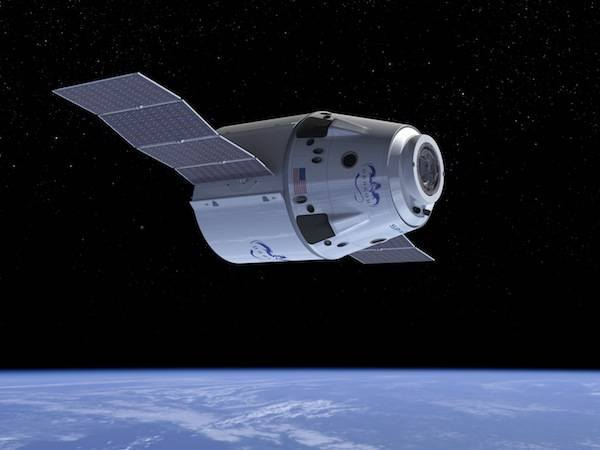
\includegraphics[height=50mm]{images/dragon}
        \end{column}
    \end{columns}
\end{frame}
}

\begin{frame}
    \frametitle{SpaceX's Future Technology}
    \begin{itemize}
        \item Send 100 people to Mars at a time
        \item Improve cost-effectiveness
        \item Make rockets reusable
    \end{itemize}

\end{frame}

\begin{frame}
    \frametitle{In practice}
    \begin{columns}
        \begin{column}{55mm}
            Achieve cost-efficiency by :
            \begin{itemize}
                \item<1-> In-house manufacturing 
                \item<2-> Innovative ideas (reusability)
                \item<3-> Using current technology
                \item<4> Saving on catering
                \item<6-> Price reaches 500 000 \$ 
            \end{itemize}
        \end{column}
        \begin{column}{65mm}
            \only<7->{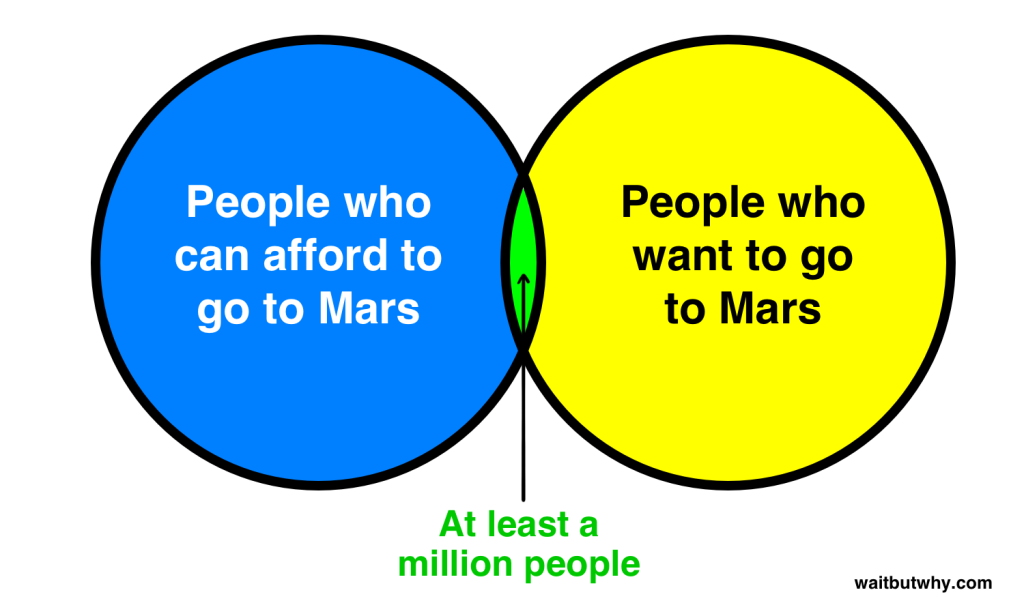
\includegraphics[width=65mm]{images/venn_mars_price}}
        \end{column}
    \end{columns}

\end{frame}


\end{document}
